\section{Results}
Table \ref{tab:ChatbotAnswers} depicts how the chatbot answered each question for each vector store. Refer to 
Table \ref{tab:GoldenDataset} for the corresponding question to each ID.

\begin{longtable}{ | p{0.05\linewidth} | p{0.2\linewidth} | p{0.2\linewidth} | p{0.2\linewidth} | p{0.2\linewidth} | }
    \hline
    \cellcolor{blue!25} ID & \cellcolor{blue!25} FAISS & \cellcolor{blue!25} SmallChunks & \cellcolor{blue!25} BigChunks & \cellcolor{blue!25}HugeChunks \\
    \hline
    \cellcolor{blue!25} 1 & \cellcolor{red!25} Wrong & \cellcolor{red!25} Wrong  
                          & \cellcolor{red!25} Wrong & \cellcolor{green!25} Correct\\
    \hline
    \cellcolor{blue!25} 2 & \cellcolor{red!25} Wrong & \cellcolor{red!25} Wrong
                          & \cellcolor{red!25} Wrong & \cellcolor{red!25} Wrong\\
    \hline 
    \cellcolor{blue!25} 3 & \cellcolor{green!25} Correct & \cellcolor{yellow!25} Questionable
                          & \cellcolor{green!25} Correct & \cellcolor{green!25} Correct\\
    \hline 
    \cellcolor{blue!25} 4 & \cellcolor{green!25} Correct & \cellcolor{yellow!25} Questionable 
                          & \cellcolor{green!25} Correct & \cellcolor{green!25} Correct \\
    \hline 
    \cellcolor{blue!25} 5 & \cellcolor{red!25} Wrong & \cellcolor{red!25} Wrong 
                          & \cellcolor{red!25} Wrong & \cellcolor{green!25} Correct\\
    \hline 
    \cellcolor{blue!25} 6 & \cellcolor{green!25} Correct & \cellcolor{green!25} Correct 
                          & \cellcolor{red!40} "I don't know" & \cellcolor{green!25} Correct\\
    \hline 
    \cellcolor{blue!25} 7 & \cellcolor{yellow!25} Questionable & \cellcolor{red!25} Wrong 
                          & \cellcolor{red!25} Wrong & \cellcolor{green!25} Correct \\
    \hline 
    \cellcolor{blue!25} 8 & \cellcolor{red!25} Wrong & \cellcolor{red!25} Wrong
                          & \cellcolor{green!25} Correct & \cellcolor{red!25} Wrong \\
    \hline
    \cellcolor{blue!25} 9 & \cellcolor{red!25} Wrong & \cellcolor{red!25} Wrong
                          & \cellcolor{red!25} Wrong & \cellcolor{green!25} Correct \\
    \hline 
    \cellcolor{blue!25} 10 & \cellcolor{green!25} Correct & \cellcolor{green!25} Correct 
                           & \cellcolor{green!25} Correct & \cellcolor{green!25} Correct\\ 
    \hline
    \cellcolor{blue!25} & \cellcolor{yellow!25} \textbf{40\%} & \cellcolor{red!25} \textbf{20\%} 
    & \cellcolor{yellow!25} \textbf{40\%} & \cellcolor{green!40} \textbf{80\%} \\
    \hline
    \caption{The performance of the chatbot with each vector store.}\label{tab:ChatbotAnswers}
\end{longtable}

\noindent Answers marked as 'Questionable' were answers that were technically correct after manual inspection despite 
GEval labelling them as incorrect. This showcases in part the occasional unreliability of LLMs even in judging contexts 
such as GEval. 

% ! Show a questionable.
% ! Perhaps 'notable observations' and talk about the IDK response and unique correct on 8 BigChunks.

\begin{figure}[H]
    \centering
    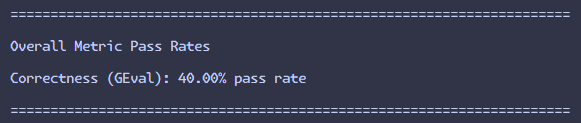
\includegraphics[width=\textwidth]{Evaluation/FAISS-HugeChunks/Overall.png}
    \caption{Overall GEval results against the "FAISS-HugeChunks" vector store (80\% correctness against expected outputs) \label{fig:EvalResults}}
\end{figure}

\noindent On the ten test cases on various academic policies and information used in evaluating the chatbot,
80\% were answered correctly according to GEval. Figures \ref{fig:WrongAnswer1} and \ref{fig:WrongAnswer2} depict 
the two queries where the chatbot failed to give a suitable answer.

\begin{figure}[H]
    \centering
    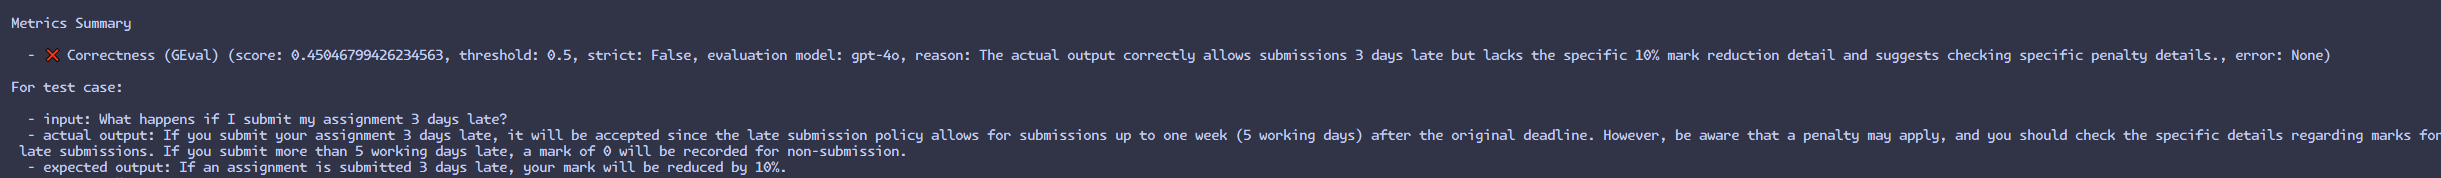
\includegraphics[width=\textwidth]{Evaluation/FAISS-HugeChunks/Incorrect1.png}
    \caption{The first incorrect answer, with the chatbot answering incorrectly. \label{fig:WrongAnswer1}}
\end{figure}

\noindent This question was answered incorrectly due to the chatbot's misinterpretation of the related policy. Work submitted up to 
1 hour after a deadline does \textbf{not} receive any grade penalty, though the chatbot likely read the following sentence: work submitted between 1 hour and 
24 hours after a deadline \textbf{does} incur a penalty. As such, this misinterpretation lead to the question being answered incorrectly.

\begin{figure}[H]
    \centering
    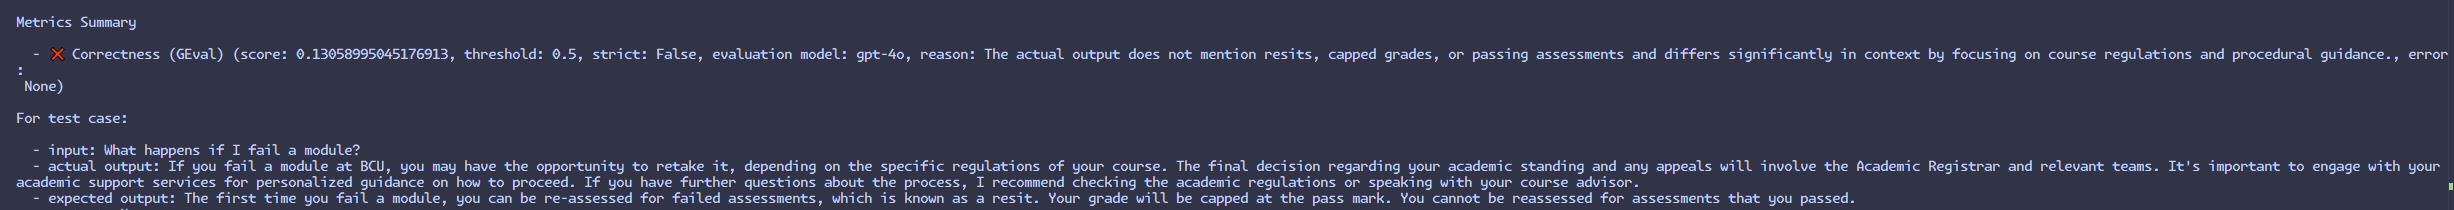
\includegraphics[width=\textwidth]{Evaluation/FAISS-HugeChunks/Incorrect2.png}
    \caption{The second incorrect answer, with incorrect information retrieval. \label{fig:WrongAnswer2}}
\end{figure}

\noindent The chatbot retrieving information that isn't directly relevant for this question implies an error in the retrieval tool. 
This could likely be due to the format of each policy document, with the information requested here (degree thresholds) being stored in
a table, depicted in Figure \ref{fig:WrongAnswer2Snippet}.

\begin{figure}[H]
    \centering
    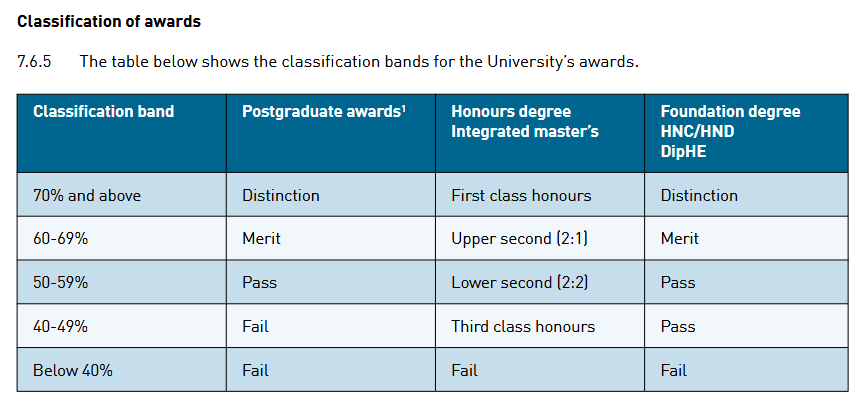
\includegraphics[width=\textwidth]{Evaluation/WrongAnswerPolicy.png}
    \caption{The snippet of the Academic Regulations that should have been referenced. \autocite{bcuPoliciesProcedures} \label{fig:WrongAnswer2Snippet}}
\end{figure}

\noindent The 'PyPDFLoader' class in LangChain, which was used when storing all University data, can sometimes misinterpret tables. 
This may in turn have created issues with the semantic search performed on the FAISS DB, leading to this question going unanswered as 
the search was unable to identify each degree classification.


\subsection{Functional requirements} 
The functional requirements, and how they were met, were as follows:

\begin{itemize}
    \item The chatbot must interpret and respond to answers in English.
    \begin{itemize}
        \item This requirement was fully met with no particular involvement from myself. OpenAI's models can automatically 
        interpret and respond with English text, as well as other languages, though other languages were not tested as I 
        cannot verify them. 
    \end{itemize}
    \item The chatbot must accept text queries.
    \begin{itemize}
        \item This was automatically met through the use of OpenAI models.
    \end{itemize}
    \item The chatbot must respond using text.
    \begin{itemize}
        \item This was automatically met through the use of OpenAI models.
    \end{itemize}
    \item The chatbot must be accessible at all times.
    \begin{itemize}
        \item When the Streamlit application is running, the chatbot can always be accessed 
        by any device connected to the same network, as long as they connect with the IP and port
        which Streamlit specifies.
    \end{itemize}
    \item The chatbot must supply BCU-related information.
    \begin{itemize}
        \item A vector database using FAISS was created containing a wide variety of BCU policies and miscellaneous
        information. Using this database, the chatbot had access to a retrieval tool which would perform a semantic 
        search on the database to retrieve BCU information relating to the user's query.
    \end{itemize}
    \item The chatbot must answer at least 75\% of BCU-related queries correctly.
    \begin{itemize}
        \item GEval reported an accuracy of 80\% against the manually produced golden answers. This is over 75\%,
        though perhaps not by a satisfactory amount. A larger testing dataset will help to provide a more accurate 
        picture in future.
    \end{itemize}
    \item The chatbot must have a GUI for ease of use and accessibility.
    \begin{itemize}
        \item Streamlit acts as the chatbot's frontend, providing a responsive and sleek UI that adapts to 
        desktop web browsers and mobile devices. The UI is simple to understand and can be navigated with the 
        Tab key on a keyboard for people unable to use a mouse.
    \end{itemize}
    \item Multiple users must be able to use the chatbot at the same time.
    \begin{itemize}
        \item Streamlit facilitates this functionality, creating isolated instances of the chatbot which do not interact 
        with each other.
    \end{itemize}
\end{itemize}

\noindent All functional requirements of the chatbot's original scope were met, producing a usable product which students 
can use to get BCU-related information at a satisfactory level of accuracy. 

\subsection{Non-functional requirements}
The non-functional requirements, and how they were met (or failed to be met) are as follows:

\begin{itemize}
    \item The chatbot should respond to queries within 10 seconds.
    \begin{itemize}
        \item All conversations with the chatbot throughout testing would gather responses 
        in fewer than 10 seconds. Queries that used RAG took significantly longer than those which 
        did not. The overall 'feel' of the app could be made faster by allowing the LLM to stream 
        text rather than output a full message, which will show the message being procedurally written 
        rather than a buffer before a full message suddenly appears.
    \end{itemize}
    \item The chatbot could allow for voice input and output.
    \begin{itemize}
        \item This requirement \textbf{was not met.} This was mostly due to time constraints, as implementing this 
        functionality would have taken substantial research that would likely not have been possible to perform 
        while meeting project deadlines. Unfortunately, this does make the app less accessible, forcing users 
        to be able to use a keyboard or have third-party voice software to input text.
    \end{itemize}
    \item The chatbot could be deployed on an existing messaging service such as Teams.
    \begin{itemize}
        \item This requirement \textbf{was not met.} As with the voice requirement, this would have taken additional 
        research and a possible redesign of the app's backend to provide an API compatible with a messaging 
        service chatbot. Given that Streamlit already provides a usable and modern UI, this requirement was instead 
        considered unnecessary.
    \end{itemize}
\end{itemize}

\noindent Only one of the three non-functional requirements was met due to time constraints which plagued development.
Even without the implementation of these features, however, the chatbot is still a very usable product.